\documentclass{article} % For LaTeX2e

\usepackage{nips14submit_e,times}
\usepackage{hyperref}
\usepackage{url}
\usepackage{graphicx}
\usepackage{booktabs}
\usepackage{listings}
\usepackage{color}

\definecolor{lightgray}{rgb}{1,1,1}
\definecolor{darkgray}{rgb}{.4,.4,.4}
\definecolor{redstrings}{rgb}{0.64,0.08,0.08}
\definecolor{blue}{rgb}{0,0,1}
\definecolor{greencomments}{rgb}{0,0.5,0}
\definecolor{cyan}{rgb}{0.0,0.6,0.6}

\renewcommand{\lstlistingname}{Code fragment}


\lstdefinelanguage{JavaScript}{
  keywords={break, case, catch, continue, debugger, default, delete, do, else, finally, for, function, if, in, instanceof, new, return, switch, this, throw, try, typeof, var, void, while, with, null},
  keywordstyle=\color{blue}\bfseries,
  ndkeywords={class, export, boolean, throw, implements, import, this},
  ndkeywordstyle=\color{blue}\bfseries,
  identifierstyle=\color{black},
  sensitive=false,
  comment=[l]{//},
  morecomment=[s]{/*}{*/},
  commentstyle=\color{greencomments}\ttfamily,
  stringstyle=\color{redstrings}\ttfamily,
  morestring=[b]',
  morestring=[b]"
}

\lstset{
   language=JavaScript,
   backgroundcolor=\color{lightgray},
   extendedchars=true,
   basicstyle=\footnotesize\ttfamily,
   showstringspaces=false,
   showspaces=false,
   numbers=left,
   numberstyle=\footnotesize,
   numbersep=9pt,
   tabsize=2,
   breaklines=true,
   showtabs=false,
   captionpos=b
}


%\documentstyle[nips14submit_09,times,art10]{article} % For LaTeX 2.09


\title{Inspecting community evolution using text and network structure}


\author{
Mario Karlovcec, Jan Rupnik, Primoz Skraba \\
Artificial Intelligence Laboratory\\
Jožef Stefan Institute\\
Jamova cesta 39, Ljubljana, Slovenia \\
}

% The \author macro works with any number of authors. There are two commands
% used to separate the names and addresses of multiple authors: \And and \AND.
%
% Using \And between authors leaves it to \LaTeX{} to determine where to break
% the lines. Using \AND forces a linebreak at that point. So, if \LaTeX{}
% puts 3 of 4 authors names on the first line, and the last on the second
% line, try using \AND instead of \And before the third author name.

\newcommand{\fix}{\marginpar{FIX}}
\newcommand{\new}{\marginpar{NEW}}

\nipsfinalcopy % Uncomment for camera-ready version

\begin{document}

\maketitle
\begin{abstract}
We propose an approach for detecting, visualizing and modelling community evolution.
Evolution is detected by applying community matching on results of statical community detection algorithms on snapshots of a dynamical network.
The approach incorporates text related to the network by extracting keywords used for evolution visualization, to show community structure and topic changes in time. Text is alongside network structure used to extract features for modelling community evolution. In this paper we build several classification and regression models and test them on the community transition prediction problem.
\end{abstract}

\section{Introduction}
In this work we propose an approach for detecting, visualizing and
modelling community evolution of dynamic networks using textual
features and graph structure. The approach is implemented in QMiner -
an open source data analytics platform for processing streams of
structured and unstructured data \footnote{http://qminer.ijs.si/}.
QMiner integrates machine learning algorithms with network analysis
based on the SNAP library \cite{snap}.


Communities in social or collaboration networks are often defined as
groups of nodes with many links inside the groups but a few links
between them. Finding communities is tantamount to looking for a
partition of the nodes that maximizes a quality function which
captures the idea of dense groups communities \cite{aynaud}. An
example of a broadly used quality function is modularity
\cite{newman2003}. However, communities are not static -- they evolve
over time, decaying, emerging, splitting and merging. Here we consider
such community dynamics, and further enrich feature set beyond the
network topology to include textual data which is available for the
primary dataset we consider -- an academic collaboration network. In particular, we use
the network topology define the communities and then use additional
information to find maps to describe how the communities evolve and
ultimately build a community evolution model where we predict the
splitting and merging of communities.


In addition to testing the accuracy of our models, we also use the
attached textual information to improve the visualization of the
communities. Using keyword extraction, we can visualize not only the
content of each community but also as see how communities evolve
through the changing associated keywords. Our approach is highly
generic and tunable. We first present the relevant previous work,
followed by a description of our approach and finally, we present the
results of experimentation on the dataset.

\section{Related work}
Standard methods for studying communities in evolving networks usually fall into three groups: (1) Static algorithms which study snapshots independently  and connect the resulting communities, (2) using temporal information directly in community detection methods and (3) using incremental/online algorithms \cite{aynaud}. In this work, we apply the first approach of independently computing communities, following by solving community matching/tracking problem to obtain the community evolution. The benefit of  the static approach is that in this context, the problemh as been  well-studied, with many different algorithms developed (for one example see Clauset-Newman-Moore\cite{clauset-newman-moore}). The main drawback is  instability \cite{aynaud2010}. When the underlying algorithms are  non-deterministic, a small modification of the input network may lead to large changes in the resulting community partition.
 
Identifying the relationships between the neighbouring partitions is often referred to as the matching or tracking problem. It is a crucial step in using static algorithms on dynamic networks as it help us identify patterns in the communities. One approach, MONIC \cite{spiliopoulou}, is a general methodology for modelling and tracking external and internal cluster transitions, that include: survival, split into multiple clusters, absorption, disappearing and emergence of a new cluster. In line with the set-theoretic approach of  the MONIC methodology, in \cite{gliwa2013} authors determine the  matching of clusters by calculating a modified Jaccard coefficient, with an additional constraint on difference in cluster sizes. Other approaches of solving the matching problem include using key nodes in the clusters \cite{wang} and community detection algorithms for the matching problem\cite{palla}. Our work includes text analysis in evolving networks, what relates to tracing topic transitions using evolution graphs in \cite{mei2005}. Predicting the future states of communities in evolving networks was done in \cite{gliwa2013}, using predictions  based on the previous events described by group size, cohesion, leadership and density.

\section{Approach}
Our approach is generic,  given a dynamic graph, each snapshot is analyzed using any statistical community detection algorithm. The detected communities are then matched and a directed graph representing community evolution is constructed. In our context, the input graph has text associated with each node. We extract keywords from the text 
 to describe the content of the communities. Finally, community evolution is visualized as a directed graph, using different colours and sizes of nodes and arcs.  Based on the extracted keywords and the graph structure, a rich feature set is constructed. We test the feature set by using it to construct a classification model for the communities.  

\begin{figure}\label{architecture}
   	\begin{center}
   	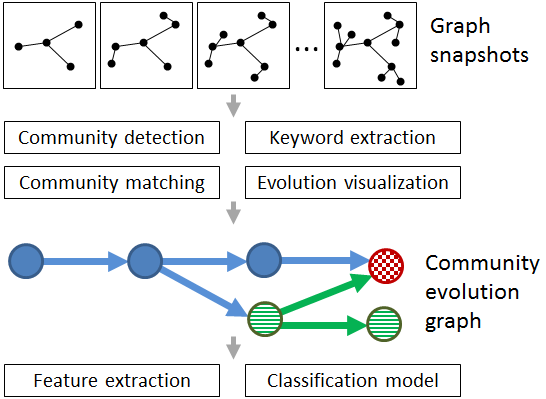
\includegraphics[width=0.5\textwidth]{architecture.png}
   	\end{center}
   	\caption{Schematic representation of the approach.}
\end{figure}
\subsection{Community detection and matching}
The input for the proposed approach is a set of snapshots of an evolving graph. A statistical community detection algorithm is applied on each snapshot. The types of supported input snapshot graphs depends on the specific community detection algorithm. These may be  undirected or directed, weighed or unweighed graphs. The approach is independent of the choice of the community detection algorithm, making it modular and applicable on the wide range of different algorithms. In our experiments we use Clauset-Newman-Moore\cite{clauset-newman-moore} algorithm. Communities as groups of members obtained from each snapshot serves as input for the community matching. The community matching problem can be reduced to determining whether a community in time $t$ exists in time $t+1$ and to which community it maps to if it exists. This is determined by calculating a modified Jaccard measure (similar as in \cite{gliwa2013})  between each pair of neighbouring communities. Let  $A$ be a community at $t$ of size $|A|$ and $B$ a community at $t+1$ of size $|B|$. The similarity measure is:
\begin{equation}
\alpha = \frac{A\cap B}{|A|},
\beta = \frac{A\cap B}{|B|}.
\end{equation}
If there are a pair of communities $A$ and $B$ such that $alpha > \tau_{alpha}$ and $beta > \tau_{beta}$, where are $\tau_{alpha}$ and $\tau_{beta}$ are two thresholds restricted to the interval $(0.5, 1]$, we say community $B$ represents the continuation of $A$ at $t+1$. Otherwise, if there is no match, community $A$ decays at $t$ and $B$ represents a new community emerged at $t+1$. Thresholds closer to 1 set stricter conditions for maintaining a cluster in the future time point. Higher value of $\tau_{alpha}$ increases the required proportion of elements in $A$ that must be retained in the same community in the future time point. $\tau_{beta}$ threshold sets the 'purity' requirement, i.e the minimum proportion of elements in B that come from A. In case $\tau_{beta} = 1$, no other elements than those from $A$ are allowed in $B$ in order to match $A$ with $B$. Restricting both thresholds to the interval $(0.5, 1]$, we ensure that each community can be matched with at most one community in the future time point. Since stability of communities can pose a difficulty in our approach, we choose $\tau_{alpha} = \tau_{alpha} = 0.5$ for the initial settings, but also experiment with other threshold values.

\subsection{Keyword extraction}
Keyword extraction process is done by first uniting textual descriptions of nodes of a community into documents. Since the members of the communities change over time, a separate document is generated for each occurrence of a community.The next step is to create bag-of-words feature space representation of the collection of documents, where each document is a vector of n-grams. Bag-of-words representations of documents are created by the standard approach involving tokenization, stop-words removal, stemming using English Porter stemmer, tf-idf weighting and normalization. The final step of the keyword extraction process is to select a number of n-grams with highest tf-idf scores from each documents.  In our experiments, we usually choose 10, since we found this is sufficient for interpreting communities. These n-grams are the keywords that represent the content of communities.

\subsection{Visualization}
An important part of this work is visualization of the community evolution. This enables quick inspection of interesting events in graph evolution, such as sudden splits and merges of communities. For example, a community with stable evolution with few communities and rear splits and merges, may at some point explode with many splits and the emergence of new communities. Such an atypical change in the structure could easily be identified with our visualization. The evolution of communities is visualized as a directed graph, with nodes representing communities and arcs showing the relationships between communities in consecutive time points. Arcs are drawn whenever two neighbouring communities share common members. The size of the nodes corresponds to the number of member of communities, while width of the arcs fits the number of shared members and is relative to the diameter of the nodes. Colour is used to indicate whether two connected neighbouring nodes represent the same community. The extracted keywords are assigned to the nodes in the directed graph, improve the interpretation of the evolution by giving context and information on the content of communities. An example of a community evolution visualization is given in Figure 2. For example, we can see how community $C$ merges with a part of community $B$ into a new community $D$.
\begin{figure}\label{evolution}
   	\begin{center}
   	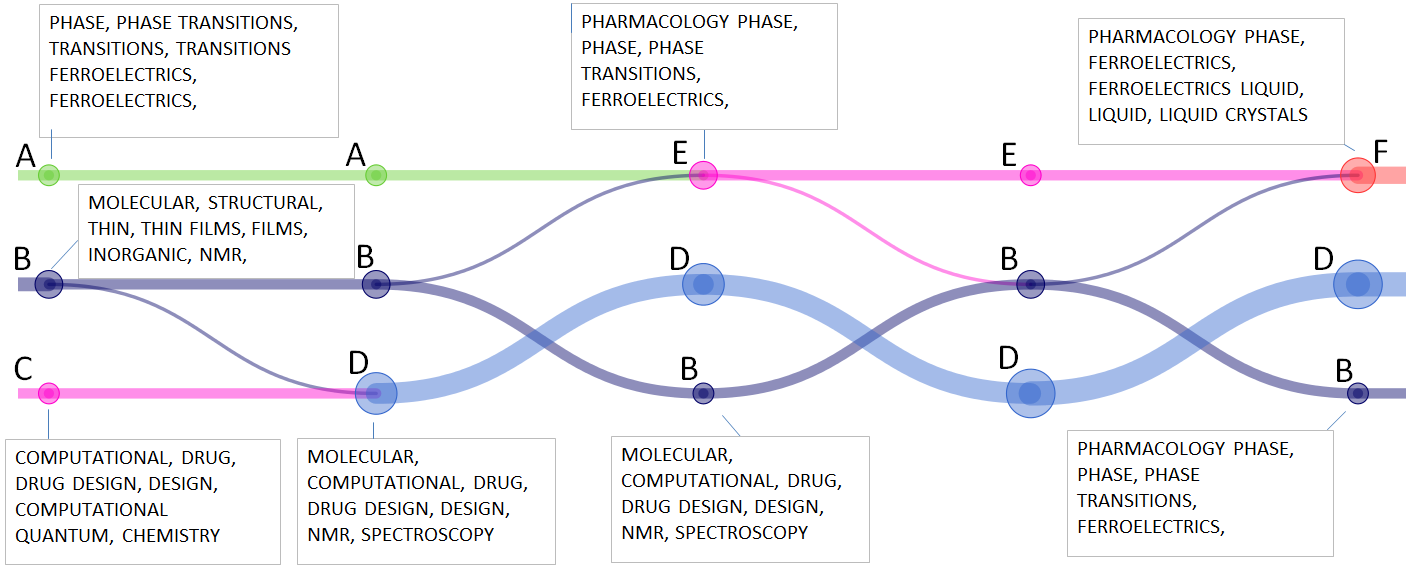
\includegraphics[width=1\textwidth]{evo.png}
   	\end{center}
   	\caption{A section of the community evolution visualization for the collaboration network in  the field of chemistry.}
\end{figure}
 
\subsection{Feature extraction}
When building our community evolution model, we use features extracted from the text assigned to communities, as well as features based on  the graph structure. The text-based features are constructed by performing text-based clustering of the community members for each time $t$ and mapping between communities and clusters. At each time,  all the members of a  community are represented using the bag-of-words feature vector representation. This process is similar to keywords extraction step, but rather than grouping the members by community, each member is represented as a separate BOW vector.  We then cluster the members based on text. If the clustering method requires a parameter for specifying the number of clusters (e.g. K-means), the number of communities at time point $t$ is used. After clustering, mapping between each community and cluster is performed. Each community gets a vector with number of elements corresponding to the number of clusters it maps to. The values of the vector are proportions of elements from a community mapped to a cluster. This vector is the basis for deriving two features: (1) {\bf the number of significant clusters it maps to} and (2) { \bf the uniformity of the mapping}. The first feature counts the number of mappings greater than a threshold restricted to the interval $[0, 1]$. In the experiments we used $K^{-1}$, where K is  the number of communities at time point $t$. The second feature, uniformity of the mapping distribution is computed using Shannon's entropy formula.

Alongside features based on text, feature set contains the five following features derived from the graph structure: (3) {\bf centralization} \cite{freeman1978}, (4) {\bf density}\cite{wasserman1994}, (5) {\bf cohesion}, (6) {\bf community age} and (7) {\bf community size}. To measure centralization, density and cohesion, a graph is constructed for each community. This is done by selecting community members and their connections as subset of nodes and edges from the snapshot in time point at which a community appears in. Centralization meausres much the connectivity of the graph depends on the most central node. It is calculated as the normalized  sum of difference in degree of the most central node and all other nodes -- centralization is the largest star structure. Density gives the number of edges with respect to  the maximal possible number of edges in the graph. Cohesion measures the connectivity of the community in relation to the connection of the community with the rest of the graph. Community age and size are derived from the community evolution directed graph and so is related to the community matching process. Age is the number of consecutive time points a community exists in the graph, while size is the number of members in the community.

\section{Experimental results}

For the purpose of evaluation, we used the co-authoring network of Slovenia researchers from the field of biotechnology from 1970 to 2013. We used a temporal resolution of 1 year to create 44 snapshots of the evolving network. The Clauset-Newman-Moore algorithm was applied for community detection, while $k$-means  was used for clustering as well as extracting text based features. We evaluated the models on two tasks: a classification task where we predicted whether a community will continue to exist in the next time point, and a regression task, where we predicted the number of communities the given community will connect to (here $1$ typically means that the community did not change). The models was evaluated in the following way. We are given a series of sets $S_t$, where $t = 0,\ldots, 43$, where the sets detail the evolution of the community structure over $43$ years. Each set $S_t$ contains examples $\{x_i, y_i, r_i)\}$, where $x_i$ is a feature vector that describes the community at time $t$, $y_i$ is a class label that encodes whether a community $i$ will split in time $t+1$, and $r_i$ corresponds to the number of communities it point to in $t+1$.

\begin{table}[h]
\caption{Results of the classification using five different classifiers}
\label{classification}
\begin{center}
\begin{tabular}{@{}llllllll@{}}
                 & accuracy & sensitivity & specificity & precision & recall & f-measure & gmean \\
                 \hline \\
decision tree    & 0.6401   & 0.7554      & 0.4917      & 0.6567    & 0.7554 & 0.7026     & 0.6094 \\
KNN              & 0.6401   & 0.7768      & 0.4641      & 0.6511    & 0.7768 & 0.7084     & 0.6004 \\
lindiscrim       & 0.6981   & \textbf{0.9056}      & 0.4309      & 0.6720    & \textbf{0.9056} & \textbf{0.7715}     & 0.6247 \\
quaddiscrim      & \textbf{0.7005}   & 0.8541      & \textbf{0.5028}      & \textbf{0.6886}    & 0.8541 & 0.7625     & \textbf{0.6553} \\
naive bayes      & 0.6787   & 0.8197      & 0.4972      & 0.6773    & 0.8197 & 0.7417     & 0.6384 \\  
\end{tabular}
\end{center}
\end{table}



\begin{table}[h]
\caption{Results of the regression using five different models}
\label{regression}
\begin{center}
\begin{tabular}{@{}llllllll@{}}
                 & RMSE & MAD & MedAD \\
                 \hline \\
regression tree	& 1.5475    & 0.8335    & 0.2222 \\
lin             & 1.3028    & 0.7597    & 0.3326  \\
glin      & 1.3028    & 0.7597    & 0.3326 \\
mean     & 1.5487    & 0.8586    & 0.3385 \\
median     & 1.6594    & 0.7585   	& 0 \\  
\end{tabular}
\end{center}
\end{table}

\noindent\textbf{Train/Test} Given the task (classification/regression) and a model, to evaluate the performance at time $t$, we aggregate all the data sets $Train_t = \bigcup_{j=1}^{t-1}{S_j}$. Then train a model on $Train_t$ and test it on the instances of $S_t$. This means that we measured a series of models (or rather an evolving model, not a single model). The testing indices ranged from $t = 24$ to $t = 43$ (which corresponds to roughly half of the dataset) in order to assure that the training sets were sufficiently large. 

\noindent\textbf{Classification:}
We evaluated the following classification algorithms\footnote{For both this and the regression models, we used
the default parameters in Matlab2013a}: classification trees,
k-nearest neighbors, linear discriminant analysis, quadratic
discriminant analysis and Naive Bayes using the normal distribution to
fit the data.
The classification performance measures include: accuracy,
sensitivity, specificity, precision, recall, f-measure and geometric
mean \emph{gmean}. 

\noindent\textbf{Regression:} We evaluated the following regression
algorithms:%\footnote{We used the default parameters in Matlab2013a}:
regression tree, linear model (least squares regression), generalized
linear model, a model that predicts the mean and a model that predicts
the median on the training set.
The following standard regression metrics were evaluated: root mean
squared error \emph{RMSE}, mean absolute deviation \emph{MAD}, median
absolute deviation \emph{MedAD}.

\section{Conclusion and discussion}
This paper gives a complete approach for detecting, visualizing and modelling evolution of communities in dynamic networks. It is based on well established statical community detection algorithms and process of community matching. This approach gives a strong importance to the text within the network. Text is used for generating keywords - summaries that describe content of the communities. These summaries are of a great value for community evolution visualization, giving an insight into both structure and topic transitions. Another important usage of text is for generating features, that are together with network structure based features used for modelling community evolution.

We have tested several classification and regression models on problem of predicting future transition of a community. Even with a small set of features, we were able to capture the community transition signal from the training examples. This points us in direction of further upgrading the model with additional text and structure based features. Since networks can significantly differ depending on the domain and content of the network, in future work we will use the text analysing compatibility in the network to detect homophily and heterophily and use this information to improve modelling. 

\subsubsection*{Acknowledgments}
   The authors gratefully acknowledge that the funding for this work was provided by the project X-LIKE (ICT-257790-STREP)\cite{xlike}.


\bibliographystyle{unsrt}
\bibliography{communities}

\end{document}